\documentclass[tikz,border=10pt]{standalone}
\usepackage{tikz}
\usetikzlibrary{calc}

\begin{document}
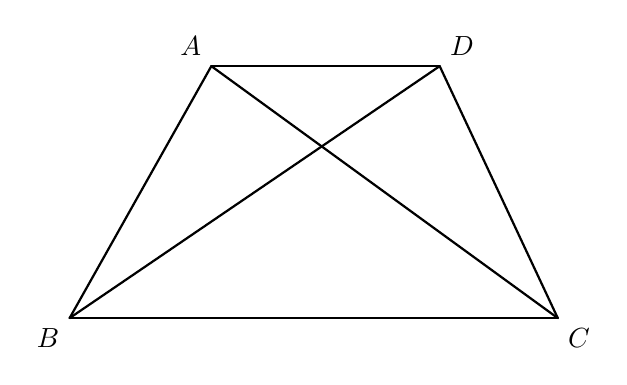
\begin{tikzpicture}[line cap=round,line join=round,thick]

\coordinate (A) at (1.8,3.2);
\coordinate (B) at (0,0);
\coordinate (C) at (6.2,0);
\coordinate (D) at (4.7,3.2);

\draw (A) -- (B);
\draw (B) -- (C);
\draw (C) -- (D);
\draw (A) -- (D);
\draw (A) -- (C);
\draw (B) -- (D);

\node[above left] at (A) {$A$};
\node[below left] at (B) {$B$};
\node[below right] at (C) {$C$};
\node[above right] at (D) {$D$};

\end{tikzpicture}
\end{document}
